\documentclass{article}
\usepackage{amssymb, amsthm, amsmath}
\usepackage{graphicx}
\usepackage{caption}

\title{Homework 3 : Logistic Regression}
\author{Elnur Gasanov : 163411}
\date{}

\parindent=0.0mm

\begin{document}

\maketitle

\section{Derivation of negative log-likelihood (NLL)}

Bernoulli distribution is used to model behaviour of the classifier, \textit{i.e.}

$$
p(t|x) = Ber(p(x)).
$$

For given $x_i$ let us denote $\mu_i$ as $p(x_i)$. Then we may rewrite the equation: $p(t_i | x_i) = \mu_i^{t_i} (1 - \mu_i)^{1 - t_i}$.

$$
likelihood = \prod_{i=1}^N p(t_i | x_i) = \prod_{i=1}^N \mu_i^{t_i} (1 - \mu_i)^{1 - t_i}.
$$

Taking negative likelihood of the above formula we get

\begin{equation*}
\boxed{NLL(w) = -\sum\limits_{i=1}^N [t_i \ln \mu_i + (1 - t_i)\ln(1 - \mu_i)]}
\end{equation*}

\section{The Gradient Descent}

Let us derive the gradient of NLL(w). Let us remind that $\mu_i = \sigma(\langle x_i, w \rangle) = \frac{1}{1 + \exp{-\langle x_i, w \rangle}}$,

$$
\frac{\partial \mu_i}{\partial w} = \frac{\exp{-\langle x_i, w \rangle}}{(1 + \exp{-\langle x_i, w \rangle})^2} \cdot x_i = \mu_i (1 - \mu_i) x_i.
$$

$$
\nabla NLL(w) = -\sum\limits_{i=1}^N \left[\frac{t_i}{\mu_i} - \frac{1 - t_i}{1 - \mu_i}\right]\frac{\partial \mu_i}{\partial w} = -\sum\limits_{i=1}^N [(1-\mu_i)t_i -\mu_i(1-t_i)]x_i = -\sum\limits_{i=1}^N [t_i-\mu_i]x_i
$$

$$
\boxed{\nabla NLL(w) = \sum\limits_{i=1}^N [\mu_i-t_i]x_i}
$$

Let us note that hessian matrix of NLL(w) $\nabla^2 NLL(w) = \sum\limits_{i=1}^N \mu_i(1-\mu_i) x_i x_i^\intercal$ is positive semidefinite. The Gradient Descent will converge to the global minimum of the problem.

\section{Sample problem}

The Gradient Descent was used to find optimal parameters of the model. Step size is $\frac{1}{\text{number of objects}}$. 

\subsection{Task 1}

The following graph of decreasing NLL values was obtained (see figure ~\ref{decreasing}).

\begin{figure}
\centering
	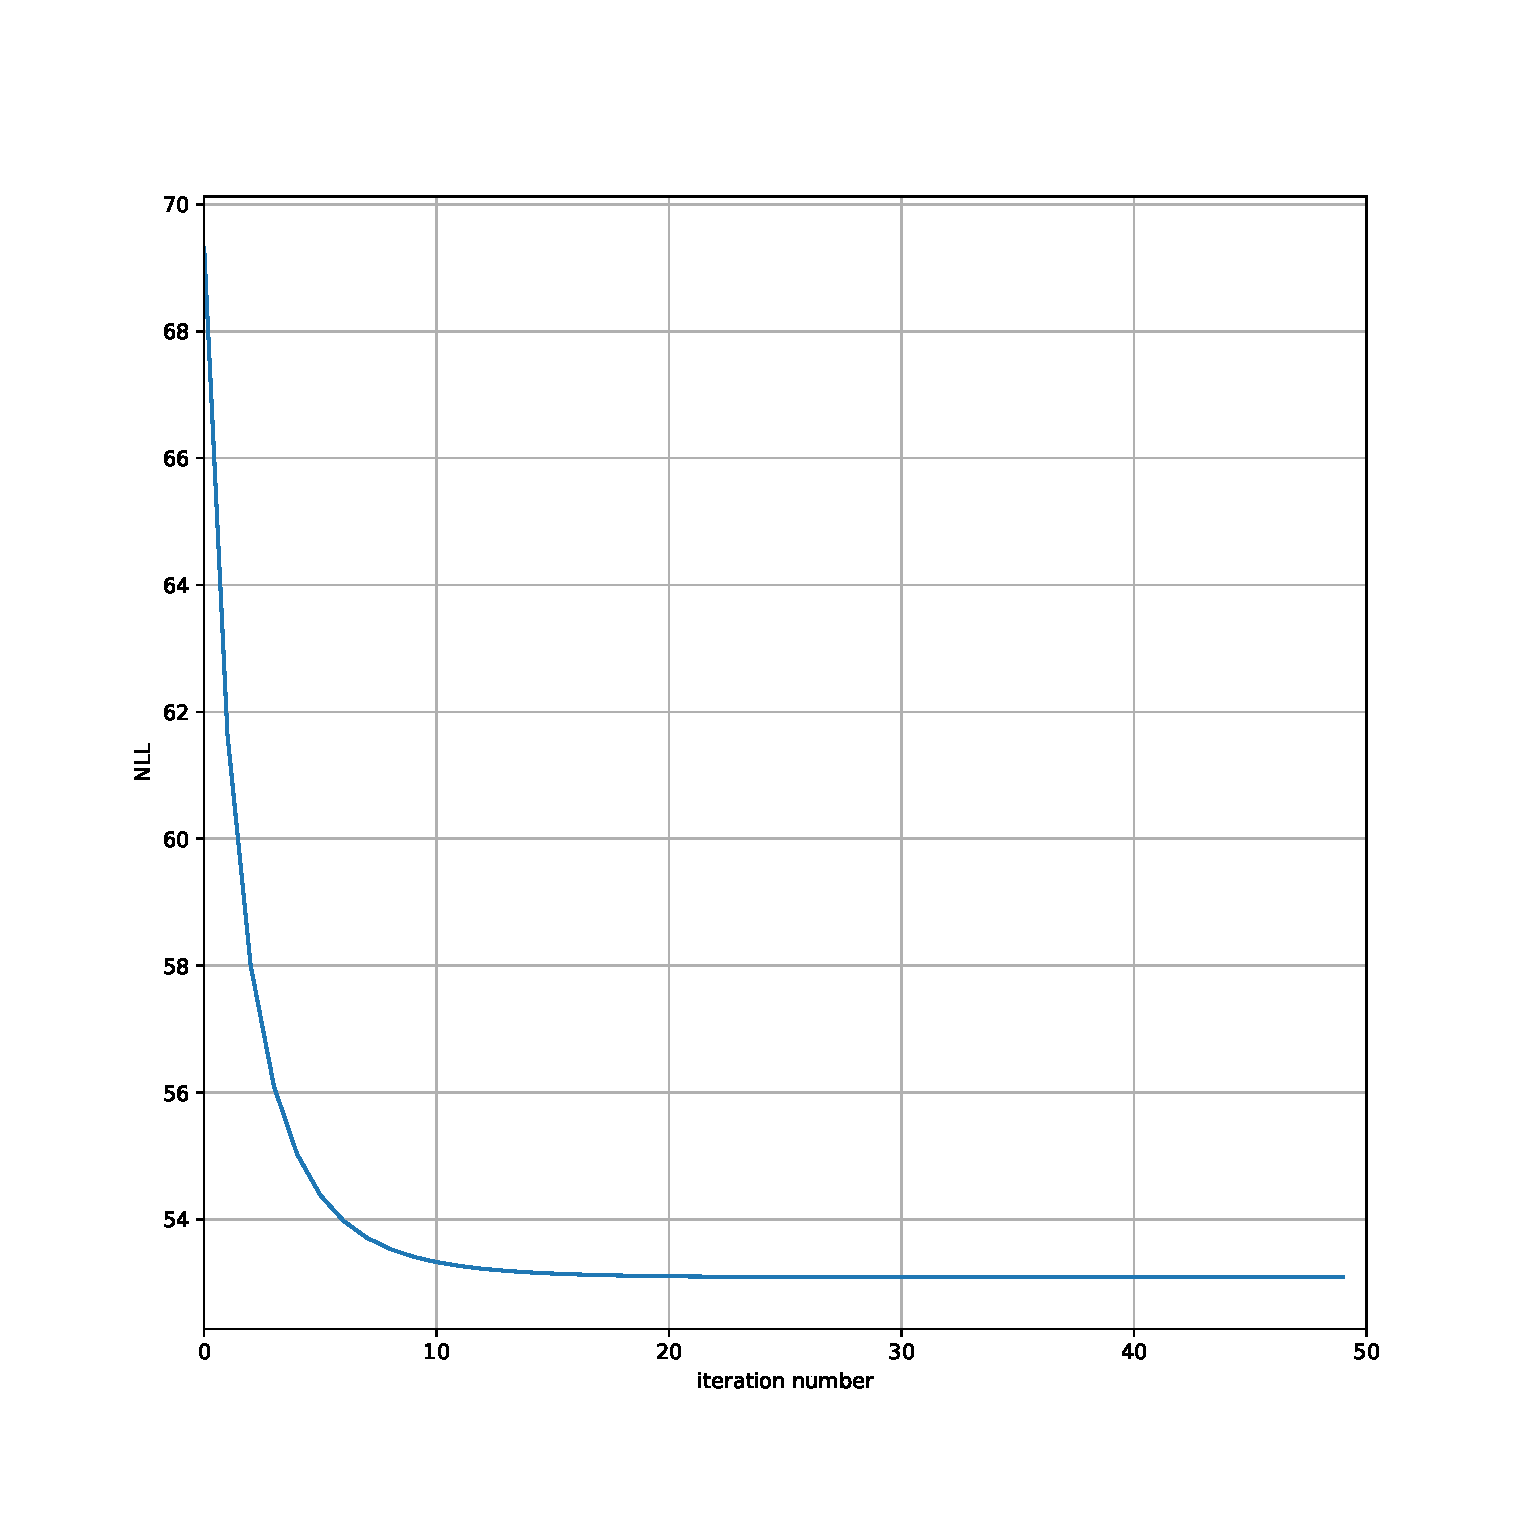
\includegraphics[width=\linewidth]{NLL_decreasing}
	\caption{Decreasing values of NLL, all features are used }\label{decreasing}
\end{figure}

We got the following optimal vector of parameters [-0.8,  0.45,  0.24,  0.81].

As we know from lectures, $\ln \frac{\mu_i}{1-\mu_i} = \langle w, x_i \rangle$. The larger value $\langle w, x_i \rangle$ is, the higher probability for an object to 'apply to graduate school'. Since $w_4 = 0.81$, we observe that GPA is an important feature. 

Launch on test data showed that 71 objects out of 100 were predicted correctly.

\subsection{Task 2}

The same work was done in task 2. Attained accuracy is {\bfseries 0.7}.

The figure \ref{gpa_plot} shows real values of target variable and values predicted by logistic regression.

What is a cutting value of GPA feature? A threshold 0.5 was used to determine the classification. 

$\frac{1}{1 + \exp-(w_0 + w_1 x_{gpa})} > 0.5 \leftrightarrow \exp-(w_0 + w_1 x_{gpa}) < 1 \leftrightarrow \boxed{x_{gpa} > -\frac{w_0}{w_1}}$. 

After multiyplying by standard deviation, adding mean of the feature we get cut-off value for GPA: 3.34.

\begin{figure*}
	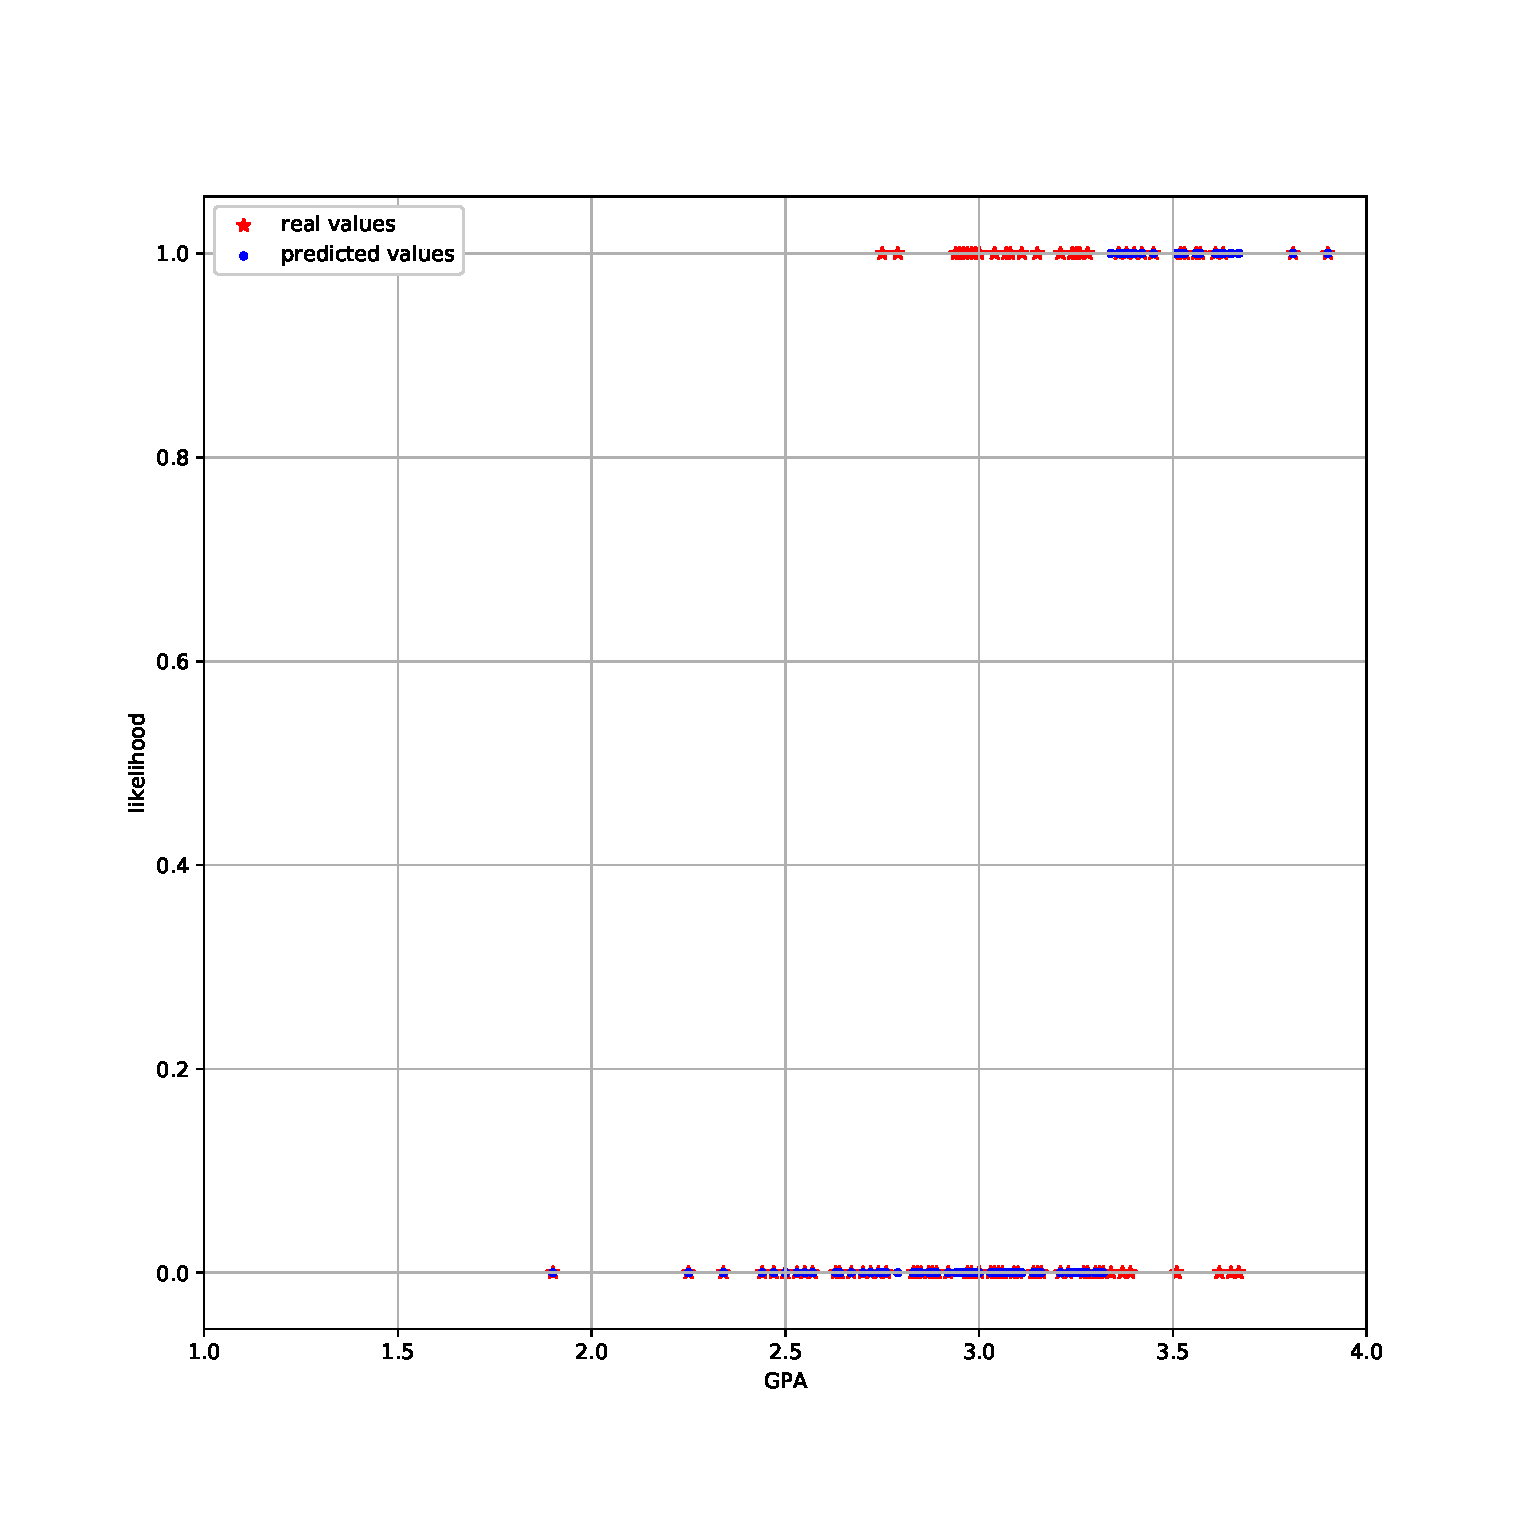
\includegraphics[width=\linewidth]{gpa_feat_plot}
	\caption{Real and predicted values in Task 2, gpa features are listed on horizontal axis}\label{gpa_plot}
\end{figure*}

\end{document}